\section{The Architecture}

This project has been implemented using ROS framework and it is a modular application that enables other nodes to query and interact with the knowledge base. Four nodes are involved in this application and the communication between them relies on an inter-process protocol handled by ROS.

\subsection{System description}

The knowledge base is loaded from the SemanticMapInterface which is a Java node based on the Jena Ontology API. This process allows requesting nodes to access and manipulate the ontology using a predefined set of operations.

\begin{figure}[H]
\centering
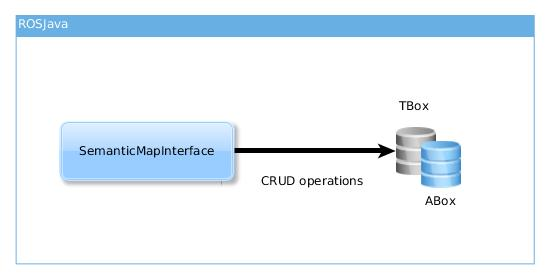
\includegraphics[width=0.8\textwidth]{imgs/semantic.jpg}
\label{fig:actions}
\caption{SemanticMapInterface Node}
\end{figure}

The exposed operations include:

\begin{itemize}
\item Loading the Terminology (TBox) and Assertion Box (ABox) into memory,
\item Listing instances, their spacial properties and their preferred lexical reference,
\item Adding a new entity of a particular class, with the spacial and lexical properties specified as arguments,
\item Updating properties of active entities,
\item Removing active entities,
\item Invoking OWL-FULL reasoner and performing inference operation given a domain model, 
\item Exporting in OWL format the list of instances present or the augmented ABox with derived properties.

\end{itemize}

The main component is the Coordinator node. This python script is an indipendent module that performs several actions and communicates with other nodes in the system. Below are listed the supported actions:

\begin{itemize}
\item Handling high level requests from other nodes such as visualizing or exporting the instances of objects present the ontology.
\item Request operations to SemanticMapInterface or to Gazebo simulator. 
\item 
\end{itemize}



\begin{figure}[H]
\centering
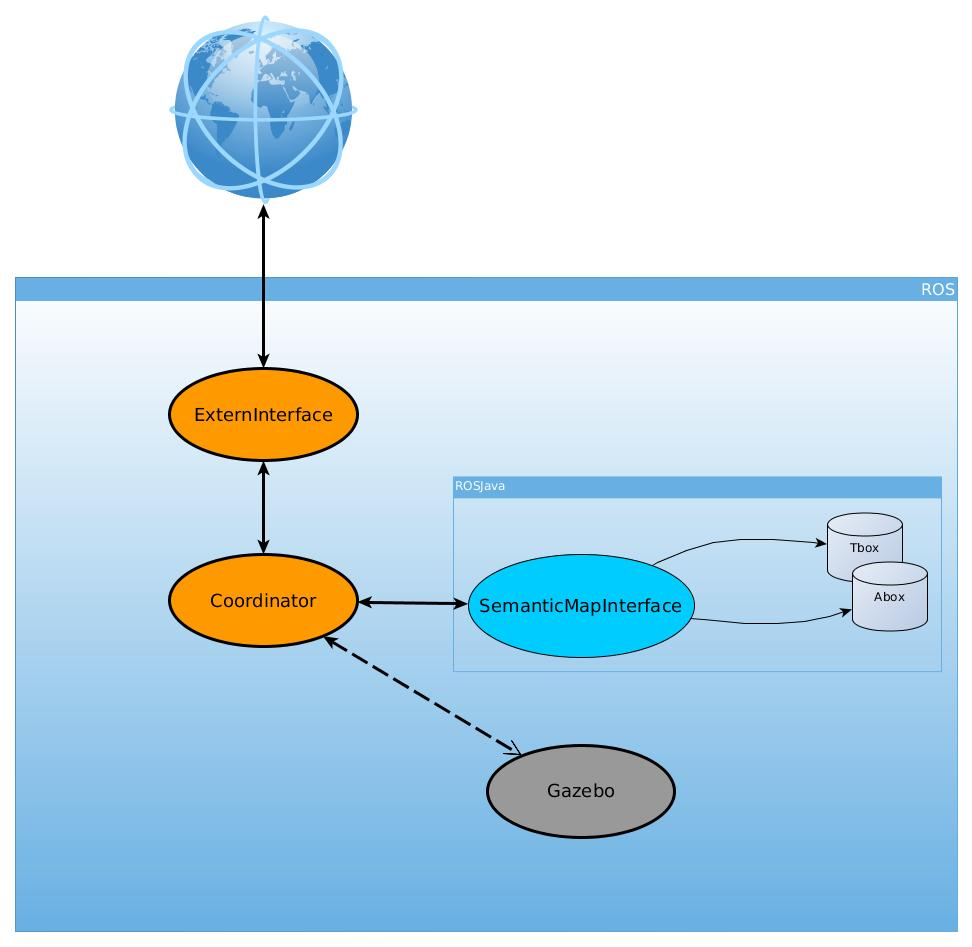
\includegraphics[width=0.8\textwidth]{imgs/architecture.jpg}
\label{fig:actions}
\caption{System Architecture}
\end{figure}


\subsection{Test case}